\documentclass[slovak]{article}
\usepackage[dvips]{graphicx}        % to include images
\usepackage{pslatex}	    % to use PostScript fonts
\usepackage[T1]{fontenc}
\usepackage[utf8]{inputenc}
\usepackage{pslatex}

\usepackage{tabularx} % tabulky na celu sirku strany
\usepackage{graphicx} %graphics files inclusion
\usepackage{longtable}
\usepackage{multirow}
\usepackage{mathtools}
\usepackage{listings}
\usepackage{pdfpages}
\usepackage{amsmath}
\usepackage{lscape}

\hyphenation{re-fe-ren-čné}
\hyphenation{de-kom-po-zí-cie}
\hyphenation{ma-xi-mál-ny}
\hyphenation{ma-xi-mál-na}
\hyphenation{al-go-rit-mus}
\hyphenation{e-xakt-né-mu}
\hyphenation{in-štan-cie}
\hyphenation{na-me-ra-ných}
\hyphenation{us-po-ria-da-ní}

\begin{document}

\title{Problém batohu - 3. úloha \\[5mm] MI-PAA, zimný semester 2014}
\author{Martin Klepáč}
\date{\today}

\maketitle

\section{Definícia problému}

Problém batohu (knapsack problem) je jeden z NP-ťažkých problémov. Pokiaľ máme k dispozícii množinu predmetov, pričom každý predmet má svoju váhu, cenu, a maximálnu nosnosť batohu, potom je naším cieľom vybrať predmety do batohu tak, aby sme maximalizovali ich cenu a pritom celková hmotnosť predmetov nepresiahla maximálnu povolenú nosnosť batohu.

\section{Formát vstupu}

Formálne, vstup vyjadríme pomocou

\begin{itemize}

\item \emph{n} = počet predmetov

\item \emph{M} = maximálna nosnosť batohu

\item \emph{vektor w} = hmotnosť jednotlivých predmetov

\item \emph{vektor c} = hodnota (cena) jednotlivých predmetov

\end{itemize}

Výstupom algoritmu je vektor \emph{x}, ktorý udáva prítomnosť/neprítomnosť daného predmetu vo výbere. Ďalej požadujeme informáciu o celkovej hmotnosti predmetov v batohu a ich súhrnú hodnotu pre najlepší výber.


\section{Úvod}

V tejto časti sa pozrieme na experimentálne vyhodnotenie výsledkov algoritmov, ktoré sme implementovali v predchádzajúcich dvoch iteráciách. Pre potreby tejto úlohy budeme uvažovať o algoritmoch dynamického programovania, branch and bound s použitím orezávania stavového priestoru a heuristika cena-váha. K tomu budeme potrebovať generátor náhodných inštancií, ktorý budeme parametrizovať tak, že v každom momente budeme meniť hodnotu práve 1 parametru a vštky ostatné zachováme konštantné.

\section{Predpoklady}

Algoritmus dynamického programania z predchádzajúcej iterácie bol založený na dekompozícii podľa kapacity. Z toho vychádza, že pokiaľ budeme meniť hodnotu kapacity batohu, doba behu algoritmu by sa mala meniť lineárne - zložitosť je závislá lineárne ako na veľkosti inštancie, tak aj na nosnosti batohu - $O(nM)$

V prípade heuristiky cena-váha neočakávam, že doba behu je závislá na akomkoľvek parametri s výnimkou usporiadanosti vstupných dát, a to z toho dôvodu, že po usporiadaní algoritmus lineárne prechádza zoznamom predmetov, až kým nedôjde k naplneniu batohu. Dalo by sa namietať, že s menšou nosnosťou batohu sa doň zmestí menší počet vecí, a teda prechod poľom usporiadaných predmetov sa zrýchli. Vzhľadom na to, že zložitosť usporiadania $O(n\log{}n)$ je rádovo vyššia ako zložitosť prechodom poľa $O(n)$, je tento faktor zanedbateľný.

Nakoniec, v prípade algoritmu branch and bound očakávam, že sa prejaví schopnosť efektívne orezať stavový priestor. To znamená, že v prípade obmedzenej nosnosti batohu voči váham predmetov dokáže algoritmus rýchlo odstrániť neperspektívne vetvy, a tým zrýchliť trvanie behu. 

V súvislosti s heuristikou cena-váha a charakterom predmetov vo výbere nie som schopný vysloviť žiadne predpoklady.

\section{Výsledky}

Školský generátor, pokiaľ nie je inak napísané, som spúšťal s nasledujúcimi parametrami:

\begin{itemize}
\item \emph{m} = 0.5
\item \emph{d} = 0
\item \emph{k} = 1
\item \emph{w-max} = 250
\item \emph{c-max} = 250
\item \emph{n} = 25
\item \emph{N} = 300
\end{itemize}

Na nasledujúcich riadkoch popíšem závislosti, ktoré som pomocou generátora objavil. Pre hore uvedenú trojicu algoritmov budem merať, ako sa mení priemerná doba behu, kým pre heuristiku cena-váha budem ďalej sledovať zmenu relatívnej chyby s meniacim sa parametrom. Závislosť na konkrétnom parametri vždy vyjadrím formou dvojice tabuliek a grafov.

V prvom kroku sme za variabilnú zložku určili \textbf{maximálnu váhu predmetu} na vstupe. Z grafu \ref{gr:graf1} je zrejmá lineárna závislosť zložitosti dynamického programovania na maximálnej váhe predmetu. Lineárna závislosť je dôsledkom dekompozície podľa kapacity batohu (viz kapitola Predpoklady) a ďalej tým, že nosnosť batohu je funkcia súčtu váh predmetov na vstupe. Trvanie metódy branch and bound a heuristiky vykazuje drobné fluktuácie, ale bez nejakého dlhodého trendu. Podobná úvaha platí pre relatívnu chybu heuristiky, ktorá sa pohybuje jemne nad pol percentom. Jemné zvýšenie rel. chyby nastáva pre \emph{w-max} sa približne rovná \emph{c-max}, t.j. vtedy keď pomer cena-váha pre jednotlivé predmety sa rovná 1. Relevantné grafy \ref{gr:graf1} a \ref{gr:graf2} a tabuľky \ref{tab1} a \ref{tab2}.

\begin{table}[htb!]\centering
	\begin{tabularx}{\textwidth}{ | X | X | X | X |}
	  \hline                       
							& \textbf{BB} 	& \textbf{DP} 	& \textbf{CV} 	\\ \hline
		\textbf{w-max=40}	&	0.002 405	&	0.000 102	&	0.000 004 020	\\ \hline
		\textbf{w-max=60}	&	0.002 726	&	0.000 153	&	0.000 004 520	\\ \hline
		\textbf{w-max=80}	&	0.002 626	&	0.000 201	&	0.000 004 600	\\ \hline
		\textbf{w-max=100}	&	0.002 750	&	0.000 249	&	0.000 004 610	\\ \hline
		\textbf{w-max=125}	&	0.002 757	&	0.000 308	&	0.000 004 620	\\ \hline
		\textbf{w-max=150}	&	0.003 343	&	0.000 353	&	0.000 004 880	\\ \hline
		\textbf{w-max=175}	&	0.002 734	&	0.000 437	&	0.000 005 090	\\ \hline
		\textbf{w-max=200}	&	0.002 957	&	0.000 507	&	0.000 005 020	\\ \hline
		\textbf{w-max=250}	&	0.002 739	&	0.000 636	&	0.000 005 330	\\ \hline
		\textbf{w-max=300}	&	0.002 606	&	0.000 765	&	0.000 005 010	\\ \hline
		\textbf{w-max=350}	&	0.002 785	&	0.000 889	&	0.000 005 310	\\ \hline
		\textbf{w-max=400}	&	0.002 653	&	0.001 025	&	0.000 005 330	\\ \hline
		\textbf{w-max=450}	&	0.002 649	&	0.001 133	&	0.000 005 150	\\ \hline								
		\textbf{w-max=500}	&	0.002 698	&	0.001 259	&	0.000 005 410	\\ \hline								
	\end{tabularx}
\caption{Závislosť trvania behu algoritmov BB,DP a heuristiky od maximálnej hmotnosti [s]}
\label{tab1}
\end{table}

\begin{table}[htb!]\centering
	\begin{tabularx}{\textwidth}{ | X | X | }
	  \hline                       
							& \textbf{CV} 	\\ \hline
		\textbf{w-max=40}	&	0.55638
			\\ \hline
		\textbf{w-max=60}	&	0.61646
			\\ \hline
		\textbf{w-max=80}	&	0.54155
			\\ \hline
		\textbf{w-max=100}	&	0.50933
			\\ \hline
		\textbf{w-max=125}	&	0.53428
			\\ \hline
		\textbf{w-max=150}	&	0.49504
			\\ \hline
		\textbf{w-max=175}	&	0.50213
			\\ \hline
		\textbf{w-max=200}	&	0.54508
			\\ \hline
		\textbf{w-max=250}	&	0.58260
			\\ \hline
		\textbf{w-max=300}	&	0.59298
			\\ \hline
		\textbf{w-max=350}	&	0.60938
			\\ \hline
		\textbf{w-max=400}	&	0.54125
			\\ \hline
		\textbf{w-max=450}	&	0.53188
			\\ \hline								
		\textbf{w-max=500}	&	0.52994
			\\ \hline								
	\end{tabularx}
\caption{Závislosť relatívnej chyby heuristiky cena/váha od maximálnej hmotnosti [\%]}
\label{tab2}
\end{table}

\begin{figure}[htb!]\centering
	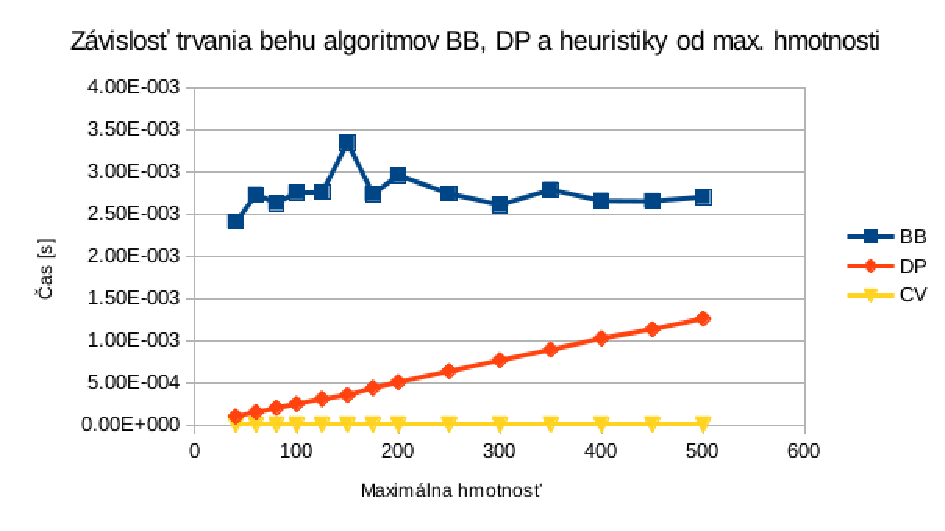
\includegraphics[scale=0.8]{./3_1.pdf}
	\caption{Závislosť trvania behu algoritmov BB, DP a heuristiky od max. hmotnosti}
	\label{gr:graf1}
\end{figure}

\begin{figure}[htb!]\centering
	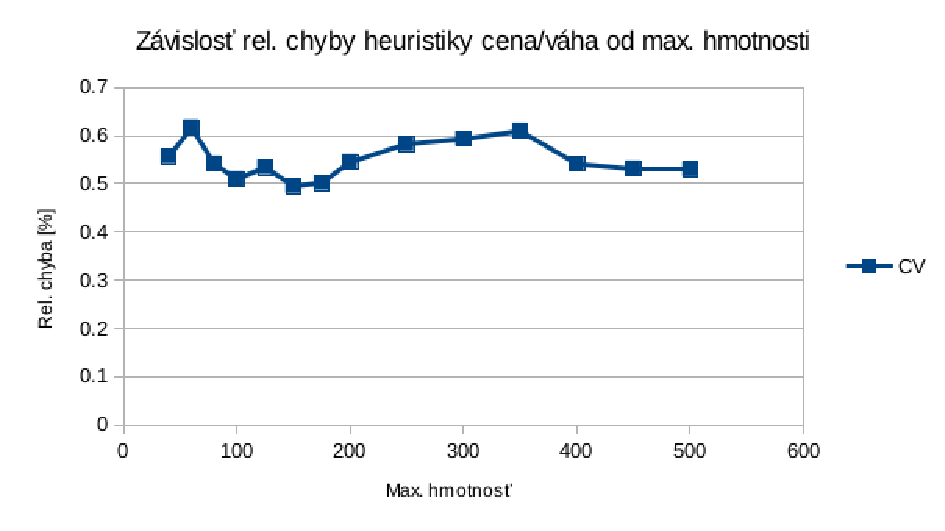
\includegraphics[scale=0.8]{./3_2.pdf}
	\caption{Závislosť rel. chyby heuristiky cena/váha od max. hmotnosti}
	\label{gr:graf2}
\end{figure}

V druhom kroku sledujeme efekt zvyšovania \textbf{maximálnej ceny predmetov}. V tomto prípade platí, že trvanie všetkých algoritmov je cenovo necitlivé. Iná situácia by nastala v prípade, ak by dynamické programovanie bolo implementované dekompozície podľa ceny. V tom prípade by sa ukázala lineárna závislosť trvania algoritmu od maximálnej ceny na vstupe, podobne ako to bolo v mojom prípade pre dekompozíciu podľa kapacity - viz predchádzajúci bod. Relatívne chyba heuristiky opäť fluktuuje mierne nad pol percentom, ale znovu sa nedá hovoriť o nejakej očividnej závislosti. Relevantné grafy \ref{gr:graf3} a \ref{gr:graf4} a tabuľky \ref{tab3} a \ref{tab4}.

\begin{table}[htb!]\centering
	\begin{tabularx}{\textwidth}{ | X | X | X | X |}
	  \hline                       
							& \textbf{BB} 	& \textbf{DP} 	& \textbf{CV} 	\\ \hline
		\textbf{c-max=40}	&	0.002 798	&	0.000 659	&	0.000 005 380	\\ \hline
		\textbf{c-max=60}	&	0.002 654	&	0.000 638	&	0.000 005 020	\\ \hline
		\textbf{c-max=80}	&	0.002 572	&	0.000 637	&	0.000 005 040	\\ \hline
		\textbf{c-max=100}	&	0.002 770	&	0.000 638	&	0.000 005 030	\\ \hline
		\textbf{c-max=125}	&	0.002 867	&	0.000 640	&	0.000 005 060	\\ \hline
		\textbf{c-max=150}	&	0.002 651	&	0.000 638	&	0.000 004 910	\\ \hline
		\textbf{c-max=175}	&	0.002 611	&	0.000 634	&	0.000 004 940	\\ \hline
		\textbf{c-max=200}	&	0.002 695	&	0.000 644	&	0.000 005 140	\\ \hline
		\textbf{c-max=250}	&	0.002 573	&	0.000 641	&	0.000 005 080	\\ \hline
		\textbf{c-max=300}	&	0.002 686	&	0.000 647	&	0.000 005 370	\\ \hline
		\textbf{c-max=350}	&	0.002 861	&	0.000 637	&	0.000 005 080	\\ \hline
		\textbf{c-max=400}	&	0.002 736	&	0.000 646	&	0.000 005 350	\\ \hline
		\textbf{c-max=450}	&	0.002 790	&	0.000 655	&	0.000 005 500	\\ \hline								
		\textbf{c-max=500}	&	0.002 686	&	0.000 650	&	0.000 005 460	\\ \hline								
	\end{tabularx}
\caption{Závislosť trvania behu algoritmov BB,DP a heuristiky od maximálnej ceny [s]}
\label{tab3}
\end{table}

\begin{table}[htb!]\centering
	\begin{tabularx}{\textwidth}{ | X | X | }
	  \hline                       
							& \textbf{CV} 	\\ \hline
		\textbf{c-max=40}	&	0.56719
			\\ \hline
		\textbf{c-max=60}	&	0.5142
			\\ \hline
		\textbf{c-max=80}	&	0.55552
			\\ \hline
		\textbf{c-max=100}	&	0.47242
			\\ \hline
		\textbf{c-max=125}	&	0.63001
			\\ \hline
		\textbf{c-max=150}	&	0.49272
			\\ \hline
		\textbf{c-max=175}	&	0.61052
			\\ \hline
		\textbf{c-max=200}	&	0.50114
			\\ \hline
		\textbf{c-max=250}	&	0.55035
			\\ \hline
		\textbf{c-max=300}	&	0.54376
			\\ \hline
		\textbf{c-max=350}	&	0.54897
			\\ \hline
		\textbf{c-max=400}	&	0.59871
			\\ \hline
		\textbf{c-max=450}	&	0.55344
			\\ \hline								
		\textbf{c-max=500}	&	0.56539
			\\ \hline								
	\end{tabularx}
\caption{Závislosť relatívnej chyby heuristiky cena/váha od maximálnej ceny [\%]}
\label{tab4}
\end{table}

V treťom kroku monitorujeme závislosť trvania behu resp. relatívnej chyby algoritmov od hodnoty prepínača generátora inštancií \emph{m}, ktorý vyjadruje \textbf{pomer medzi kapacitou batohu a súčtom váh} predmetov na vstupe. Graf \ref{gr:graf6} ukazuje klesajúcu chybu heuristiky v závislosti od narastajúceho pomeru. Teda, čím sa do batohu zmestí relatívne väčší počet predmetov, tým je chyba heuristiky nižšia (limitne sa blíži k nule, pretože každý predmet sa do batohu zlepší). Dynamické programovanie vykazuje lineárny rast - opäť je to spôsobené lineárne sa zvyšujúcou kapacitou batohu, podobne ako tomu bolo pri maximálnej váhe. Algoritmus branch and bound dokáže pri nízkom pomere kapacity batohu a sume váh predmetov efektívne orezať statový priestor, ale táto vlastnosť sa s narastajúcim pomerom zhoršuje, čoho výsledkom je exponenciálny rast doby behu pre nízke \emph{m}. Relevantné grafy \ref{gr:graf5} a \ref{gr:graf6} a tabuľky \ref{tab5} a \ref{tab6}.

\begin{figure}[htb!]\centering
	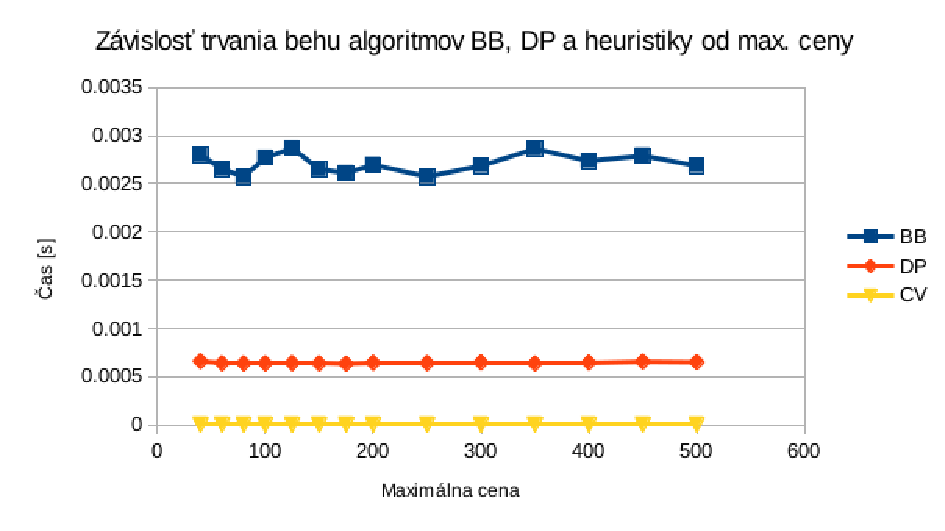
\includegraphics[scale=0.8]{./3_3.pdf}
	\caption{Závislosť trvania behu algoritmov BB. DP a heuristiky od max. ceny }
	\label{gr:graf3}
\end{figure}

\begin{figure}[htb!]\centering
	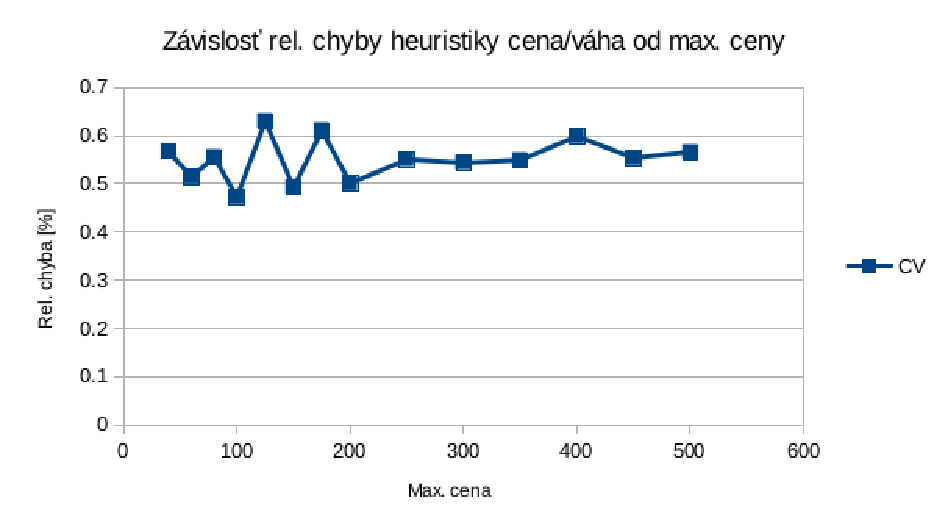
\includegraphics[scale=0.8]{./3_4.pdf}
	\caption{Závislosť rel. chyby heuristiky cena/váha od max. ceny}
	\label{gr:graf4}
\end{figure}

\begin{table}[htb!]\centering
	\begin{tabularx}{\textwidth}{ | X | X | X | X |}
	  \hline                       
							& \textbf{BB} 	& \textbf{DP} 	& \textbf{CV} 	\\ \hline
		\textbf{pomer=0.1}	&	0.000 039		&		0.000 1055		&	0.000 003 880			\\ \hline
		\textbf{pomer=0.2}	&	0.000 143		&		0.000 2274		&	0.000 003 950			\\ \hline
		\textbf{pomer=0.3}	&	0.000 447		&		0.000 3523		&	0.000 004 120			\\ \hline
		\textbf{pomer=0.4}	&	0.001 156		&		0.000 4783		&	0.000 004 170			\\ \hline
		\textbf{pomer=0.5}	&	0.002 673		&		0.000 6507		&	0.000 005 520			\\ \hline
		\textbf{pomer=0.6}	&	0.004 853		&		0.000 7976		&	0.000 006 050			\\ \hline
		\textbf{pomer=0.7}	&	0.007 638		&		0.000 9356		&	0.000 006 200			\\ \hline
		\textbf{pomer=0.8}	&	0.009 888		&		0.001 0469		&	0.000 006 060			\\ \hline
		\textbf{pomer=0.9}	&	0.010 618		&		0.001 1860		&	0.000 006 360			\\ \hline
	\end{tabularx}
\caption{Závislosť trvania behu algoritmov BB,DP a heuristiky od pomeru nosnosť/suma váh [s]}
\label{tab5}
\end{table}

\begin{table}[htb!]\centering
	\begin{tabularx}{\textwidth}{ | X | X | }
	  \hline                       
							& \textbf{CV} 	\\ \hline
		\textbf{pomer=0.1}	&	1.4738
			\\ \hline
		\textbf{pomer=0.2}	&	1.0519
			\\ \hline
		\textbf{pomer=0.3}	&	0.97004
			\\ \hline
		\textbf{pomer=0.4}	&	0.78315
			\\ \hline
		\textbf{pomer=0.5}	&	0.49983
			\\ \hline
		\textbf{pomer=0.6}	&	0.3608
			\\ \hline
		\textbf{pomer=0.7}	&	0.22867
			\\ \hline
		\textbf{pomer=0.8}	&	0.17306
			\\ \hline
		\textbf{pomer=0.9}	&	0.084475
			\\ \hline
	\end{tabularx}
\caption{Závislosť relatívnej chyby heuristiky cena/váha od pomeru nosnosť batohu/suma váh [\%]}
\label{tab6}
\end{table}

\begin{figure}[htb!]\centering
	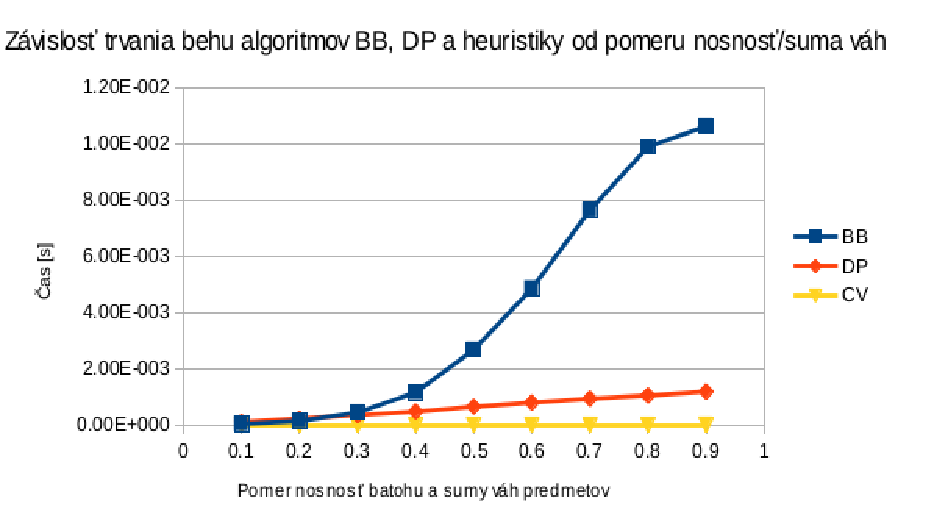
\includegraphics[scale=0.8]{./3_5.pdf}
	\caption{Závislosť trvania behu algoritmov BB, DP a heuristiky od pomeru nosnosť vs. suma váh}
	\label{gr:graf5}
\end{figure}

\begin{figure}[htb!]\centering
	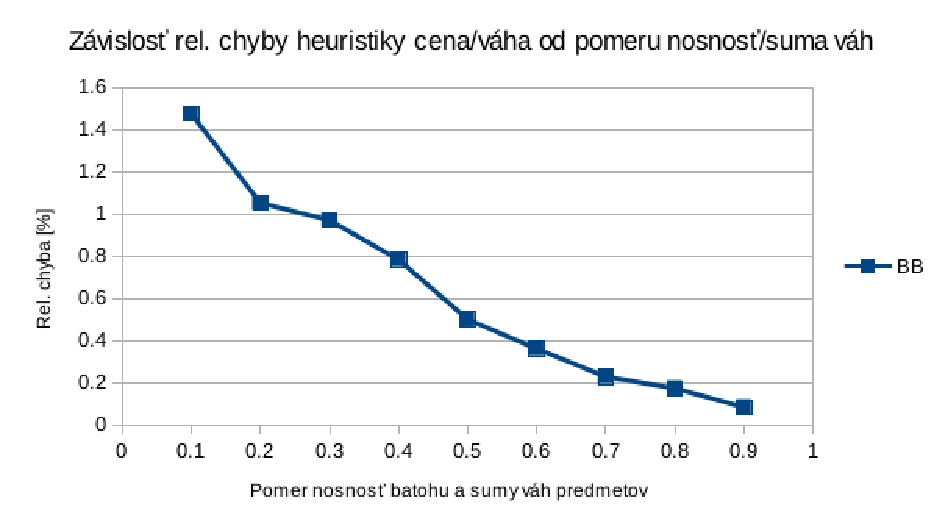
\includegraphics[scale=0.8]{./3_6.pdf}
	\caption{Závislosť rel. chyby heuristiky cena/váha od pomeru nosnosť/suma váh}
	\label{gr:graf6}
\end{figure}

Ako posledný faktor budeme meniť \textbf{granularitu dát} pomocou parametra \emph{k} pre prevahu veľkých vecí (\emph{d=1}). Platí, že čím väčšia hodnota tohto parametra, tým je menšia pravdepodobnosť malých dát na vstupe. Z toho vyplýva, že so zvyšujúcim sa počtom veľkých predmetov (narastajúce \emph{k}) rastie zároveň aj nosnosť batohu, a teda opäť dochádza k rastu doby behu metódy dynamického programovania. Naopak, doba behu algoritmu branch and bound klesá približne exponenciálne s narastajúcim počtom veľkých predmetov na vstupe až do fázy, v ktorej beží rýchlejšie ako dynamické programovanie. Beh heuristiky, ako tomu bolo vo všetkých predchádzajúcich prípadoch, nie je závislý na granularite vstupných dát. S narastajúcou hodnotou váh predmetov ale dochádza k zmenšovaniu relatívnych chýb až k hodnote 0.1 percenta. Relevantné grafy \ref{gr:graf7} a \ref{gr:graf8} a tabuľky \ref{tab7} a \ref{tab8}.

\begin{table}[htb!]\centering
	\begin{tabularx}{\textwidth}{ | X | X | X | X |}
	  \hline                       
							& \textbf{BB} 	& \textbf{DP} 	& \textbf{CV} 	\\ \hline
		\textbf{exp=0.1}	&	0.002 830		&	0.000 755		&	0.000 005 560			\\ \hline
		\textbf{exp=0.2}	&	0.002 815		&	0.000 770		&	0.000 005 580			\\ \hline
		\textbf{exp=0.4}	&	0.002 304		&	0.000 828		&	0.000 005 350			\\ \hline
		\textbf{exp=0.6}	&	0.001 931		&	0.000 939		&	0.000 005 480			\\ \hline
		\textbf{exp=0.8}	&	0.001 636		&	0.001 026		&	0.000 005 460			\\ \hline
		\textbf{exp=1}		&	0.001 269		&	0.001 076		&	0.000 005 380			\\ \hline
		\textbf{exp=1.5}	&	0.000 972		&	0.001 185		&	0.000 005 440			\\ \hline
		\textbf{exp=2}		&	0.000 800		&	0.001 259		&	0.000 005 600			\\ \hline
		\textbf{exp=2.5}	&	0.000 785		&	0.001 321		&	0.000 005 360			\\ \hline
		\textbf{exp=3}		&	0.000 754		&	0.001 301		&	0.000 005 550			\\ \hline
		\textbf{exp=4}		&	0.000 665		&	0.001 197		&	0.000 004 760			\\ \hline
	\end{tabularx}	
\caption{Závislosť trvania behu algoritmov BB,DP a heuristiky od exponentu granularity [s]}
\label{tab7}
\end{table}

\begin{table}[htb!]\centering
	\begin{tabularx}{\textwidth}{ | X | X | }
	  \hline                       
							& \textbf{CV} 	\\ \hline
		\textbf{exp=0.1}	&	0.57106
			\\ \hline
		\textbf{exp=0.2}	&	0.55837
			\\ \hline
		\textbf{exp=0.4}	&	0.56664
			\\ \hline
		\textbf{exp=0.6}	&	0.53169
			\\ \hline
		\textbf{exp=0.8}	&	0.61671
			\\ \hline
		\textbf{exp=1}		&	0.53568
			\\ \hline
		\textbf{exp=1.5}	&	0.45679
			\\ \hline
		\textbf{exp=2}		&	0.45407
			\\ \hline
		\textbf{exp=2.5}	&	0.14103
			\\ \hline
		\textbf{exp=3}		&	0.29805
			\\ \hline
		\textbf{exp=4}		&	0.12878
			\\ \hline
	\end{tabularx}
\caption{Závislosť relatívnej chyby heuristiky cena/váha od exponentu granularity [\%]}
\label{tab8}
\end{table}

\begin{figure}[htb!]\centering
	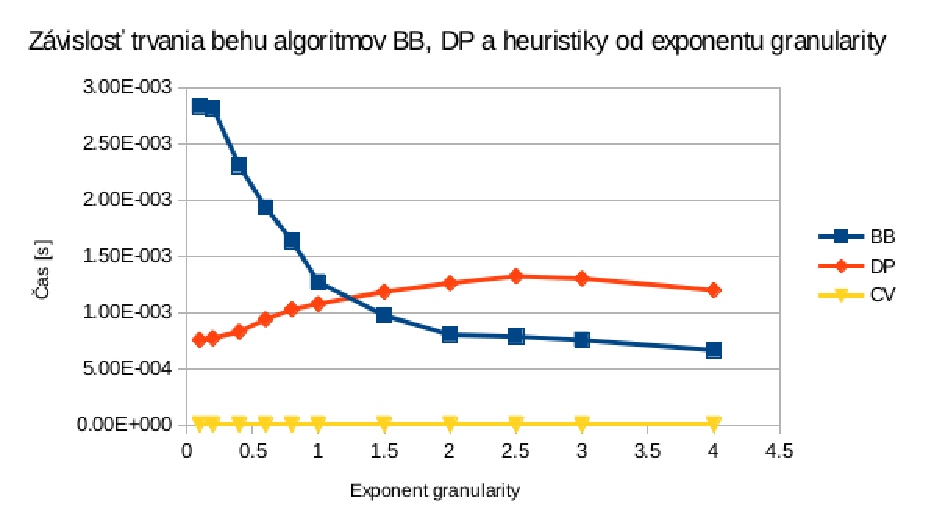
\includegraphics[scale=0.8]{./3_7.pdf}
	\caption{Závislosť trvania behu algoritmov BB, DP a heuristiky od exponentu granularity}
	\label{gr:graf7}
\end{figure}

\begin{figure}[htb!]\centering
	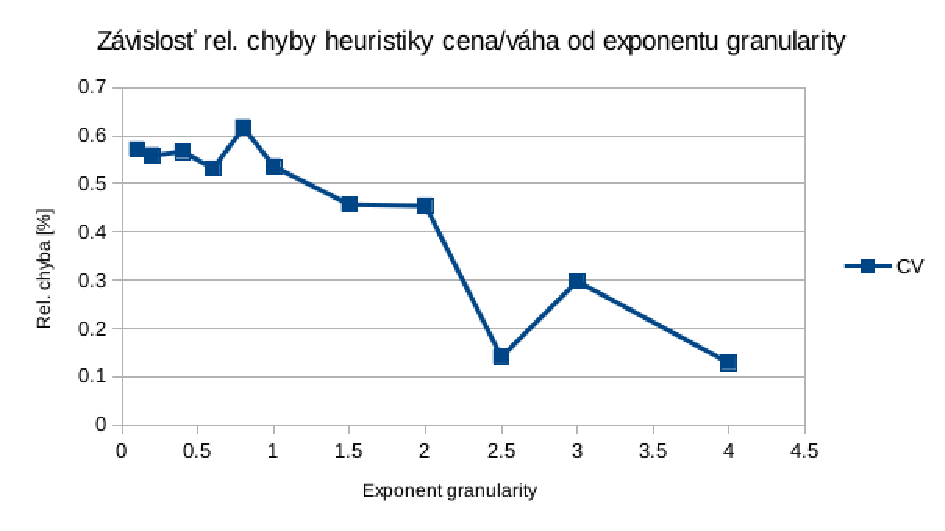
\includegraphics[scale=0.8]{./3_8.pdf}
	\caption{Závislosť rel. chyby cena/váha od exponentu granularity}
	\label{gr:graf8}
\end{figure}

\section{Zhodnotenie}

\begin{table}[htb!]\centering
	\begin{tabularx}{\textwidth}{ | X | X | X | X |}
	  \hline                       
		\textbf{Algoritmus}			& \textbf{Presnosť} 	& \textbf{Rýchlosť} 	& \textbf{Hodnotenie} 	\\ \hline
		\textbf{Brute force}		& absolútna				&	pomalá (exponenciálna)		&	poskytuje exaktné, referenčné riešenie, nepoužiteľné pre väčšie inštancie 			\\ \hline
		\textbf{Dynamické programovanie (dekompozícia podľa kapacity)}		& absolútna				&	rýchla (pseudopolynomálna)		&	pamäťovo náročná, závislá na hmotnosti predmetov			\\ \hline
		\textbf{Branch and bound}	& absolútna				&	rýchla, ale závislá na charaktere vstupných dát (v najhoršom prípade rovnaká ako brute force)	& 	efektívna pokiaľ kapacita batohu výrazne menšia ako suma váh predmetov		\\ \hline
		\textbf{Heuristika cena-váha}& vysoká (chyba maximálne v rámci jednotiek percent)				&	rýchla, nezávislá od charakteru vstupných dát		&	efektívna, ak sa do batohu zmestí veľké percento predmetov			\\ \hline
	\end{tabularx}	
\caption{Porovnanie implementovaných algoritmov}
\label{tab9}
\end{table}

\end{document}
